\chapter{評価}
\label{evaluation}
本章では,提案システムの評価について述べる.

\section{評価方法}
倉庫棚を模した棚にQRコードを貼り付け\ref{course},実際に想定した経路を飛行できるかを確認した.
また,本手法の特徴として毎回QRコードの前で位置の補正を行う為他の手法よりも巡回に時間がかかる物と考えられる.
そこで,コースを巡回させ続け位置補正に要する時間を100回分計測した.
実際には以下のコースを用いて計測した.


\begin{figure}[htbp]
  \begin{center}
    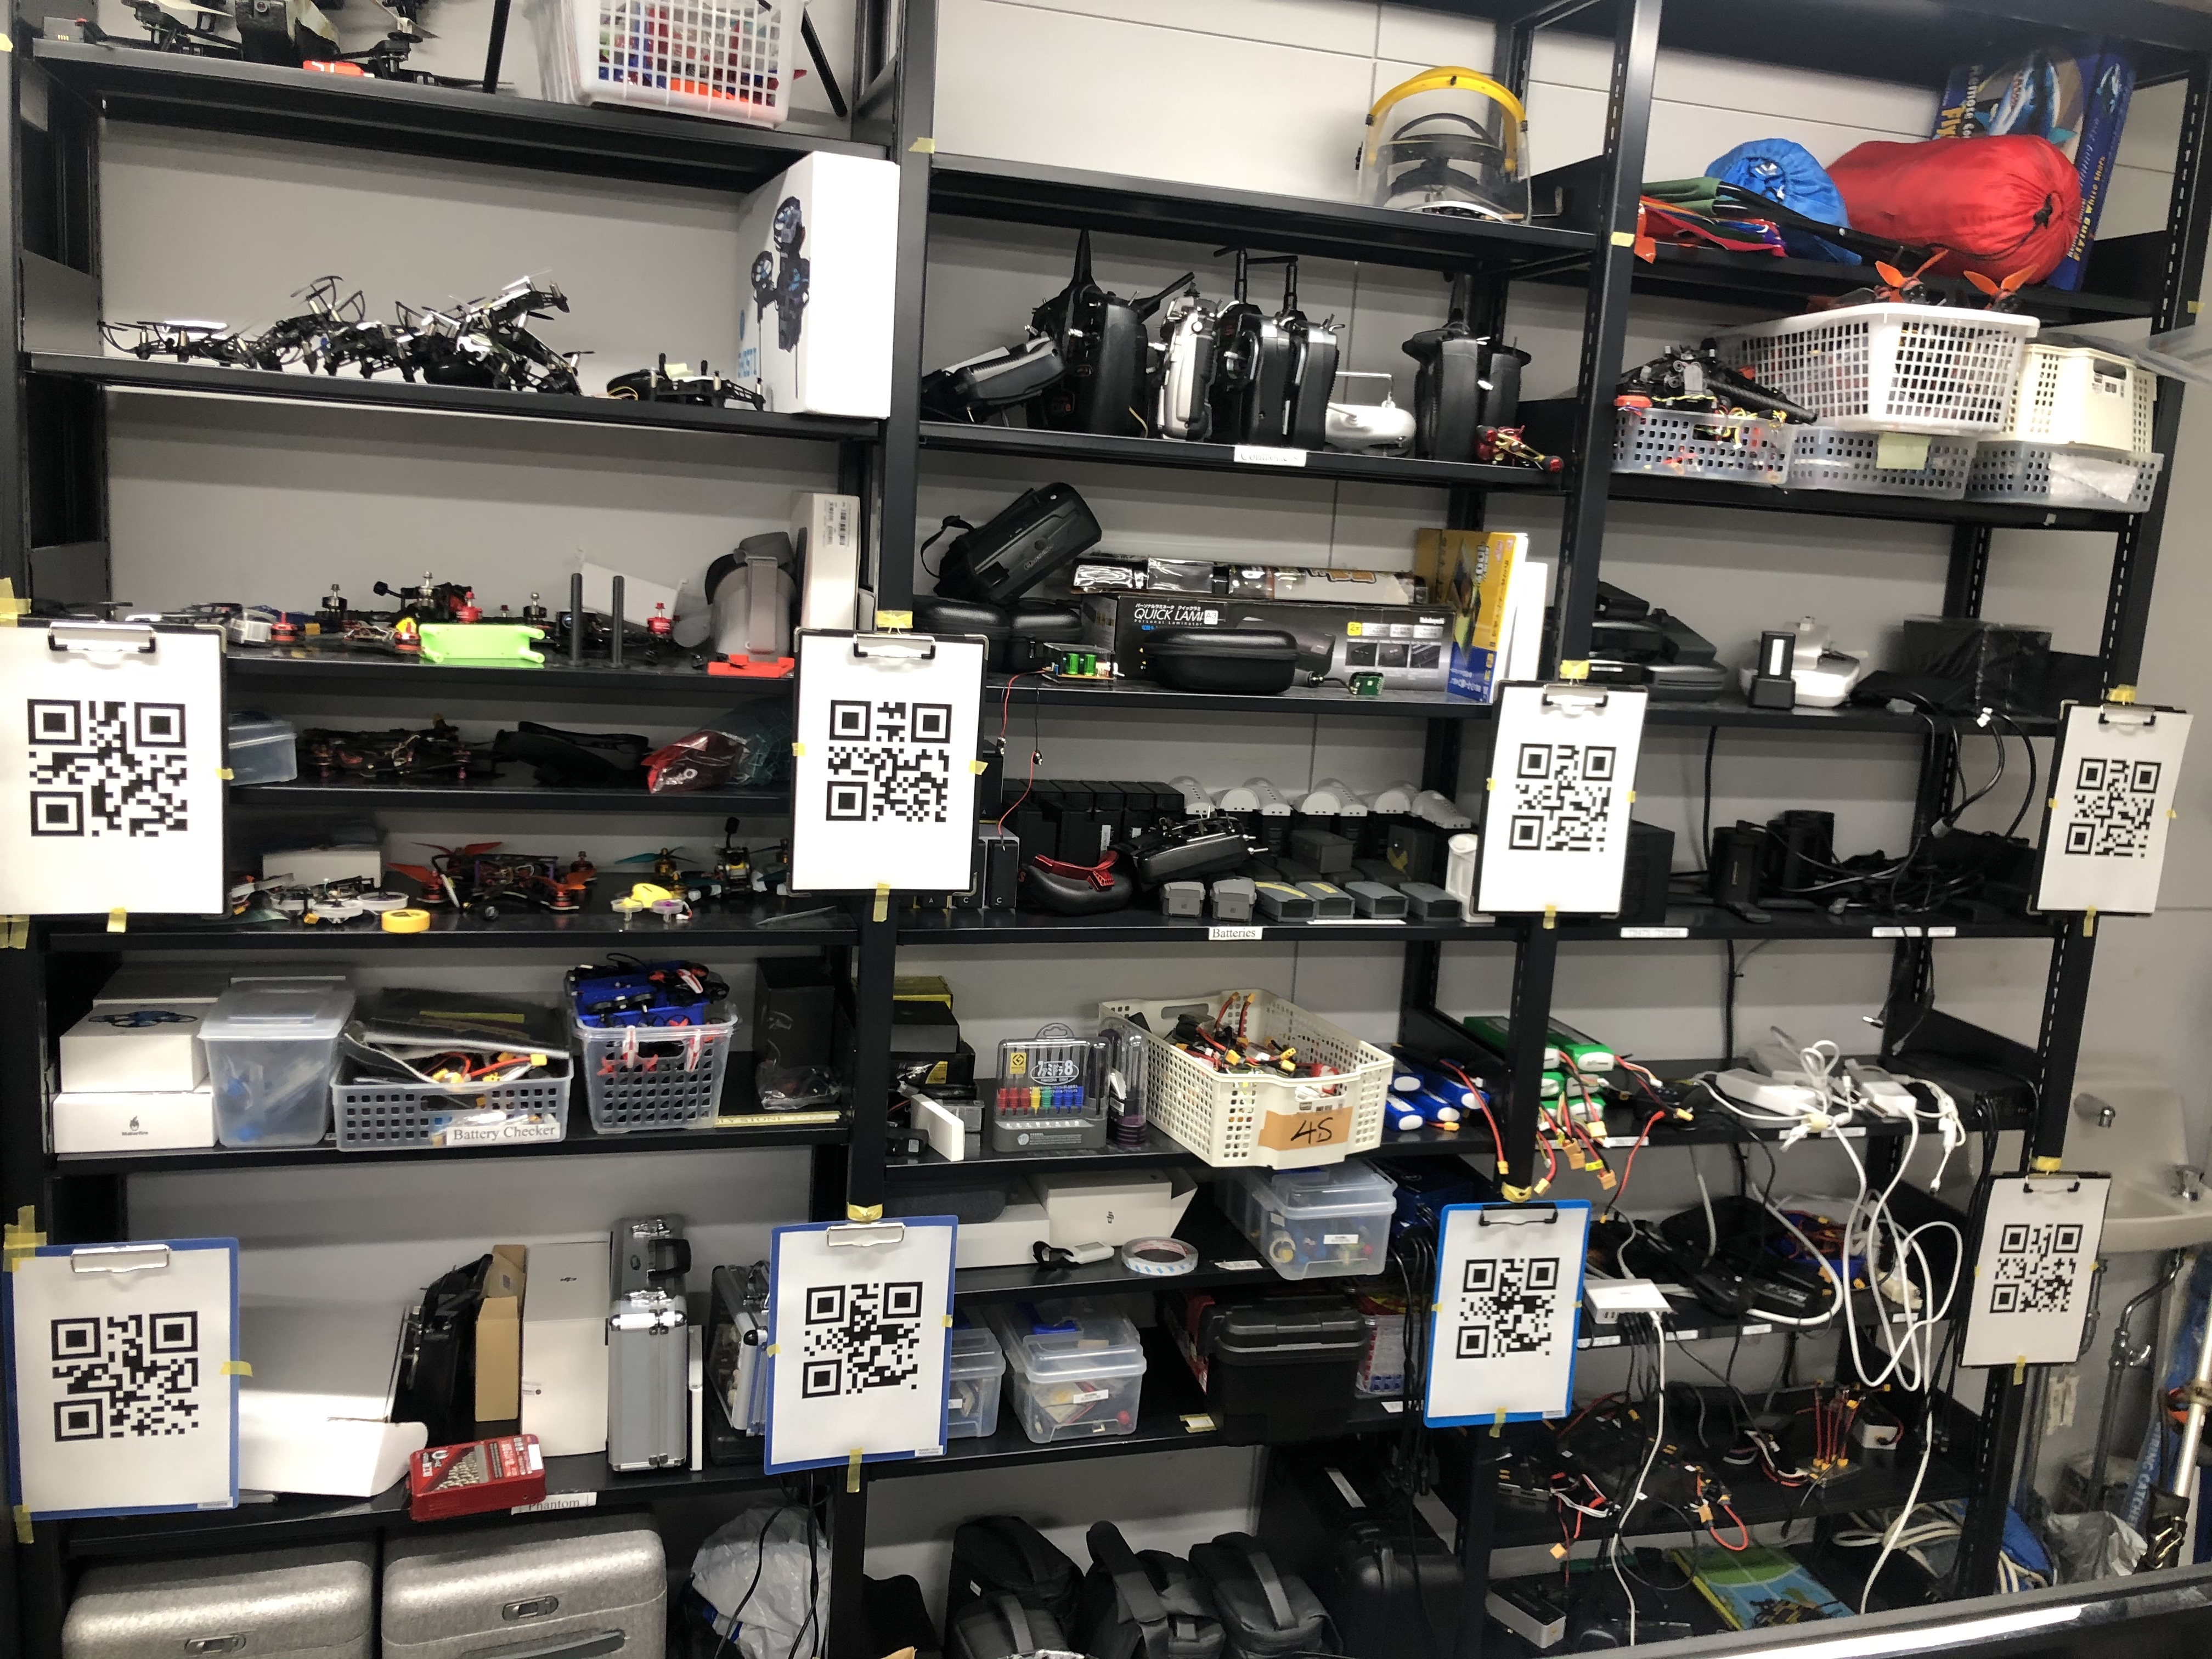
\includegraphics[clip,width=15.0cm]{img/course.jpg}
    \caption{評価用コース}
    \label{course}
  \end{center}
\end{figure}

また,QRコードにはそれぞれ以下の情報が文字列で保存されている
\begin{enumerate}
    \item {x: 80}
    \item {x: 90}
    \item {x: 90}
    \item {y: 70}
    \item {x: -90}
    \item {x: -90}
    \item {x: -80}
    \item {y: -70}
\end{enumerate}

今回は使用機材の解像度の都合上QRコードに対して距離85cmを維持するようにした.


%%% Local Variables:
%%% mode: japanese-latex
%%% TeX-master: "./thesis"
%%% End:
